% Options for packages loaded elsewhere
\PassOptionsToPackage{unicode}{hyperref}
\PassOptionsToPackage{hyphens}{url}
%
\documentclass[
]{article}
\usepackage{lmodern}
\usepackage{amssymb,amsmath}
\usepackage{ifxetex,ifluatex}
\ifnum 0\ifxetex 1\fi\ifluatex 1\fi=0 % if pdftex
  \usepackage[T1]{fontenc}
  \usepackage[utf8]{inputenc}
  \usepackage{textcomp} % provide euro and other symbols
\else % if luatex or xetex
  \usepackage{unicode-math}
  \defaultfontfeatures{Scale=MatchLowercase}
  \defaultfontfeatures[\rmfamily]{Ligatures=TeX,Scale=1}
\fi
% Use upquote if available, for straight quotes in verbatim environments
\IfFileExists{upquote.sty}{\usepackage{upquote}}{}
\IfFileExists{microtype.sty}{% use microtype if available
  \usepackage[]{microtype}
  \UseMicrotypeSet[protrusion]{basicmath} % disable protrusion for tt fonts
}{}
\makeatletter
\@ifundefined{KOMAClassName}{% if non-KOMA class
  \IfFileExists{parskip.sty}{%
    \usepackage{parskip}
  }{% else
    \setlength{\parindent}{0pt}
    \setlength{\parskip}{6pt plus 2pt minus 1pt}}
}{% if KOMA class
  \KOMAoptions{parskip=half}}
\makeatother
\usepackage{xcolor}
\IfFileExists{xurl.sty}{\usepackage{xurl}}{} % add URL line breaks if available
\IfFileExists{bookmark.sty}{\usepackage{bookmark}}{\usepackage{hyperref}}
\hypersetup{
  pdftitle={GDP Structure Analysis},
  pdfauthor={Kate Chalmers \& Hicham Moustaine},
  hidelinks,
  pdfcreator={LaTeX via pandoc}}
\urlstyle{same} % disable monospaced font for URLs
\usepackage[margin=1in]{geometry}
\usepackage{color}
\usepackage{fancyvrb}
\newcommand{\VerbBar}{|}
\newcommand{\VERB}{\Verb[commandchars=\\\{\}]}
\DefineVerbatimEnvironment{Highlighting}{Verbatim}{commandchars=\\\{\}}
% Add ',fontsize=\small' for more characters per line
\usepackage{framed}
\definecolor{shadecolor}{RGB}{248,248,248}
\newenvironment{Shaded}{\begin{snugshade}}{\end{snugshade}}
\newcommand{\AlertTok}[1]{\textcolor[rgb]{0.94,0.16,0.16}{#1}}
\newcommand{\AnnotationTok}[1]{\textcolor[rgb]{0.56,0.35,0.01}{\textbf{\textit{#1}}}}
\newcommand{\AttributeTok}[1]{\textcolor[rgb]{0.77,0.63,0.00}{#1}}
\newcommand{\BaseNTok}[1]{\textcolor[rgb]{0.00,0.00,0.81}{#1}}
\newcommand{\BuiltInTok}[1]{#1}
\newcommand{\CharTok}[1]{\textcolor[rgb]{0.31,0.60,0.02}{#1}}
\newcommand{\CommentTok}[1]{\textcolor[rgb]{0.56,0.35,0.01}{\textit{#1}}}
\newcommand{\CommentVarTok}[1]{\textcolor[rgb]{0.56,0.35,0.01}{\textbf{\textit{#1}}}}
\newcommand{\ConstantTok}[1]{\textcolor[rgb]{0.00,0.00,0.00}{#1}}
\newcommand{\ControlFlowTok}[1]{\textcolor[rgb]{0.13,0.29,0.53}{\textbf{#1}}}
\newcommand{\DataTypeTok}[1]{\textcolor[rgb]{0.13,0.29,0.53}{#1}}
\newcommand{\DecValTok}[1]{\textcolor[rgb]{0.00,0.00,0.81}{#1}}
\newcommand{\DocumentationTok}[1]{\textcolor[rgb]{0.56,0.35,0.01}{\textbf{\textit{#1}}}}
\newcommand{\ErrorTok}[1]{\textcolor[rgb]{0.64,0.00,0.00}{\textbf{#1}}}
\newcommand{\ExtensionTok}[1]{#1}
\newcommand{\FloatTok}[1]{\textcolor[rgb]{0.00,0.00,0.81}{#1}}
\newcommand{\FunctionTok}[1]{\textcolor[rgb]{0.00,0.00,0.00}{#1}}
\newcommand{\ImportTok}[1]{#1}
\newcommand{\InformationTok}[1]{\textcolor[rgb]{0.56,0.35,0.01}{\textbf{\textit{#1}}}}
\newcommand{\KeywordTok}[1]{\textcolor[rgb]{0.13,0.29,0.53}{\textbf{#1}}}
\newcommand{\NormalTok}[1]{#1}
\newcommand{\OperatorTok}[1]{\textcolor[rgb]{0.81,0.36,0.00}{\textbf{#1}}}
\newcommand{\OtherTok}[1]{\textcolor[rgb]{0.56,0.35,0.01}{#1}}
\newcommand{\PreprocessorTok}[1]{\textcolor[rgb]{0.56,0.35,0.01}{\textit{#1}}}
\newcommand{\RegionMarkerTok}[1]{#1}
\newcommand{\SpecialCharTok}[1]{\textcolor[rgb]{0.00,0.00,0.00}{#1}}
\newcommand{\SpecialStringTok}[1]{\textcolor[rgb]{0.31,0.60,0.02}{#1}}
\newcommand{\StringTok}[1]{\textcolor[rgb]{0.31,0.60,0.02}{#1}}
\newcommand{\VariableTok}[1]{\textcolor[rgb]{0.00,0.00,0.00}{#1}}
\newcommand{\VerbatimStringTok}[1]{\textcolor[rgb]{0.31,0.60,0.02}{#1}}
\newcommand{\WarningTok}[1]{\textcolor[rgb]{0.56,0.35,0.01}{\textbf{\textit{#1}}}}
\usepackage{graphicx,grffile}
\makeatletter
\def\maxwidth{\ifdim\Gin@nat@width>\linewidth\linewidth\else\Gin@nat@width\fi}
\def\maxheight{\ifdim\Gin@nat@height>\textheight\textheight\else\Gin@nat@height\fi}
\makeatother
% Scale images if necessary, so that they will not overflow the page
% margins by default, and it is still possible to overwrite the defaults
% using explicit options in \includegraphics[width, height, ...]{}
\setkeys{Gin}{width=\maxwidth,height=\maxheight,keepaspectratio}
% Set default figure placement to htbp
\makeatletter
\def\fps@figure{htbp}
\makeatother
\setlength{\emergencystretch}{3em} % prevent overfull lines
\providecommand{\tightlist}{%
  \setlength{\itemsep}{0pt}\setlength{\parskip}{0pt}}
\setcounter{secnumdepth}{-\maxdimen} % remove section numbering

\title{GDP Structure Analysis}
\author{Kate Chalmers \& Hicham Moustaine}
\date{11/25/2020}

\begin{document}
\maketitle

\hypertarget{estimation-outlier-removal}{%
\subsubsection{Estimation \& Outlier
Removal}\label{estimation-outlier-removal}}

A simple OLS regression is run in order to evaluate how well our sample
of country explains Morocco's 2020 Q2 GDP growth.

Breaking down GDP into 12 contributing sub-sectors by country, we
regress the average value of these sectors first onto GDP to see how
well the model fits overall.

The following countries are included in our estimation:

\begin{Shaded}
\begin{Highlighting}[]
\KeywordTok{unique}\NormalTok{(tot.wide}\OperatorTok{$}\NormalTok{country)}
\end{Highlighting}
\end{Shaded}

\begin{verbatim}
##  [1] "Austria"        "Belgium"        "Bulgaria"       "Colombia"       "Costa Rica"    
##  [6] "Czechia"        "Denmark"        "Estonia"        "Finland"        "France"        
## [11] "Germany"        "Greece"         "Hungary"        "India"          "Ireland"       
## [16] "Italy"          "Latvia"         "Lithuania"      "Luxembourg"     "Netherlands"   
## [21] "Norway"         "Poland"         "Portugal"       "Romania"        "Slovakia"      
## [26] "Slovenia"       "South Korea"    "Spain"          "Sweden"         "Switzerland"   
## [31] "Tunisia"        "Turkey"         "Ukraine"        "United Kingdom"
\end{verbatim}

The first regression is the full set of countries, excluding Morocco to
avoid multi-colinearity issues. We also drop Egypt from our estimation,
but would like to keep it in mind later on in case we would like to
evaluate robustness through its inclusion.

\begin{Shaded}
\begin{Highlighting}[]
\NormalTok{full.set<-}\KeywordTok{lm}\NormalTok{(gdp }\OperatorTok{~}\StringTok{ }\NormalTok{agri }\OperatorTok{+}\StringTok{ }\NormalTok{cons }\OperatorTok{+}\StringTok{ }\NormalTok{trade }\OperatorTok{+}\StringTok{ }\NormalTok{fin }\OperatorTok{+}\StringTok{ }\NormalTok{industry }\OperatorTok{+}\StringTok{ }\NormalTok{info }\OperatorTok{+}\StringTok{ }\NormalTok{manuf }\OperatorTok{+}\StringTok{ }\NormalTok{other }\OperatorTok{+}\StringTok{ }\NormalTok{tech }\OperatorTok{+}\StringTok{ }\NormalTok{public }\OperatorTok{+}\StringTok{ }\NormalTok{estate }\OperatorTok{+}\StringTok{ }\NormalTok{services, }\DataTypeTok{data=}\NormalTok{tot.wide)}

\KeywordTok{summary}\NormalTok{(full.set)}
\end{Highlighting}
\end{Shaded}

\begin{verbatim}
## 
## Call:
## lm(formula = gdp ~ agri + cons + trade + fin + industry + info + 
##     manuf + other + tech + public + estate + services, data = tot.wide)
## 
## Residuals:
##      Min       1Q   Median       3Q      Max 
## -2.16780 -0.33209  0.02167  0.46888  2.16933 
## 
## Coefficients:
##              Estimate Std. Error t value Pr(>|t|)    
## (Intercept) -1.077751   0.798769  -1.349 0.192330    
## agri         0.009737   0.011375   0.856 0.402120    
## cons        -0.027547   0.016780  -1.642 0.116297    
## trade        0.087425   0.047924   1.824 0.083093 .  
## fin          0.145743   0.034768   4.192 0.000449 ***
## industry     0.287506   0.050530   5.690 1.44e-05 ***
## info         0.174891   0.045401   3.852 0.000994 ***
## manuf       -0.007683   0.039043  -0.197 0.845975    
## other       -0.014737   0.010192  -1.446 0.163678    
## tech         0.003927   0.034165   0.115 0.909642    
## public      -0.091518   0.073815  -1.240 0.229385    
## estate       0.030948   0.037415   0.827 0.417909    
## services     0.340527   0.189296   1.799 0.087142 .  
## ---
## Signif. codes:  0 '***' 0.001 '**' 0.01 '*' 0.05 '.' 0.1 ' ' 1
## 
## Residual standard error: 1.193 on 20 degrees of freedom
##   (1 observation deleted due to missingness)
## Multiple R-squared:  0.9759, Adjusted R-squared:  0.9614 
## F-statistic: 67.49 on 12 and 20 DF,  p-value: 1.777e-13
\end{verbatim}

It is useful to note that the R-squared is very high so our model does
fit the data well. But the relationship between sectors is only weakly
significant. This could be influenced by the outliers that we noted in
our analysis. So we can try removing observations to see how this
improves the model.

We run some quick plots to evaluate linearity and check those with high
standard deviations to decide which values to drop.

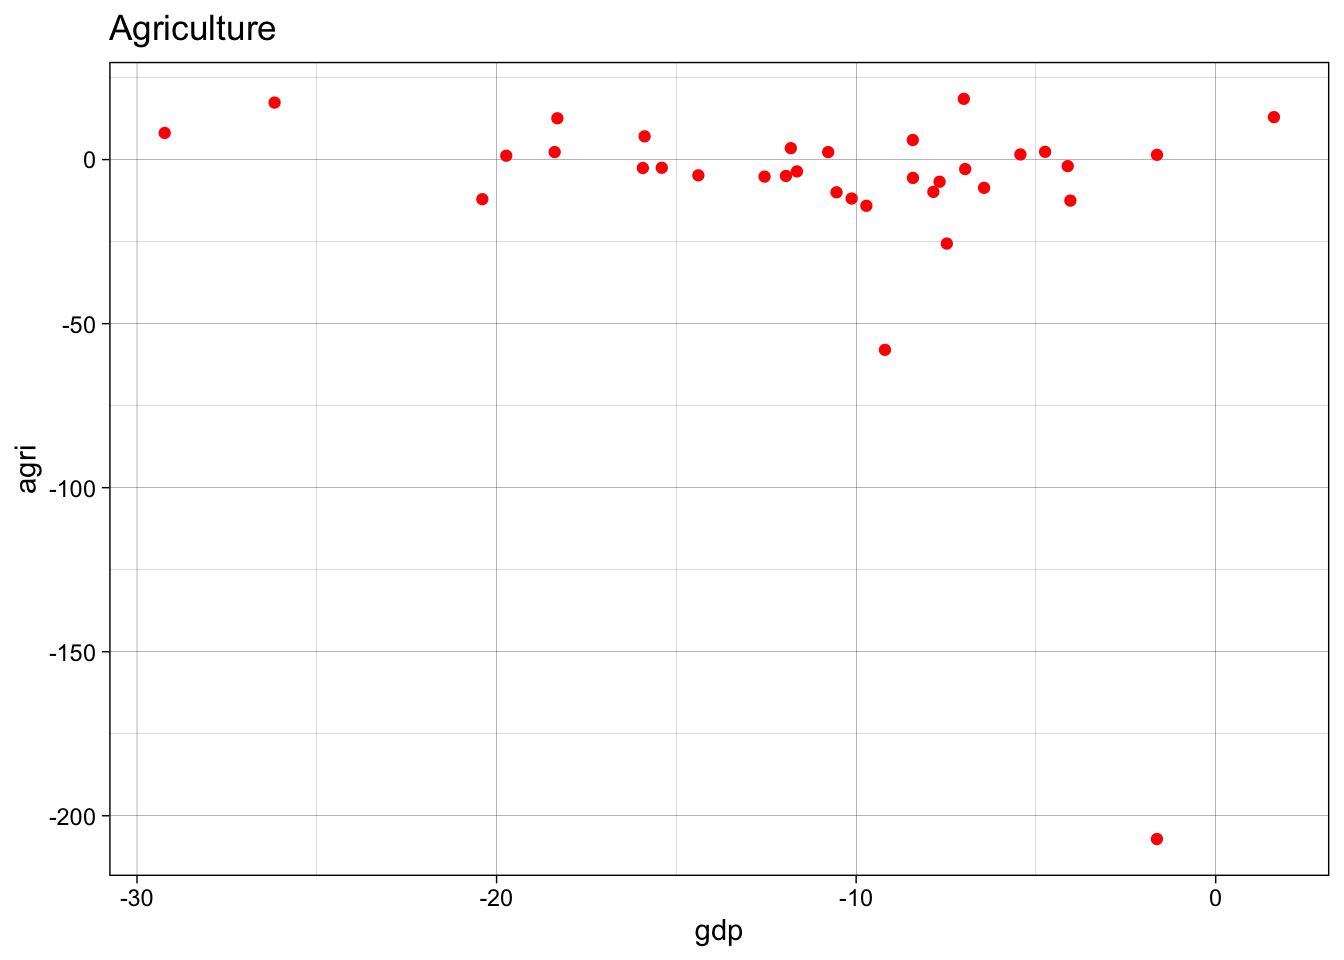
\includegraphics[width=0.33\linewidth]{Morocco_GDP_prediction_files/figure-latex/unnamed-chunk-1-1}
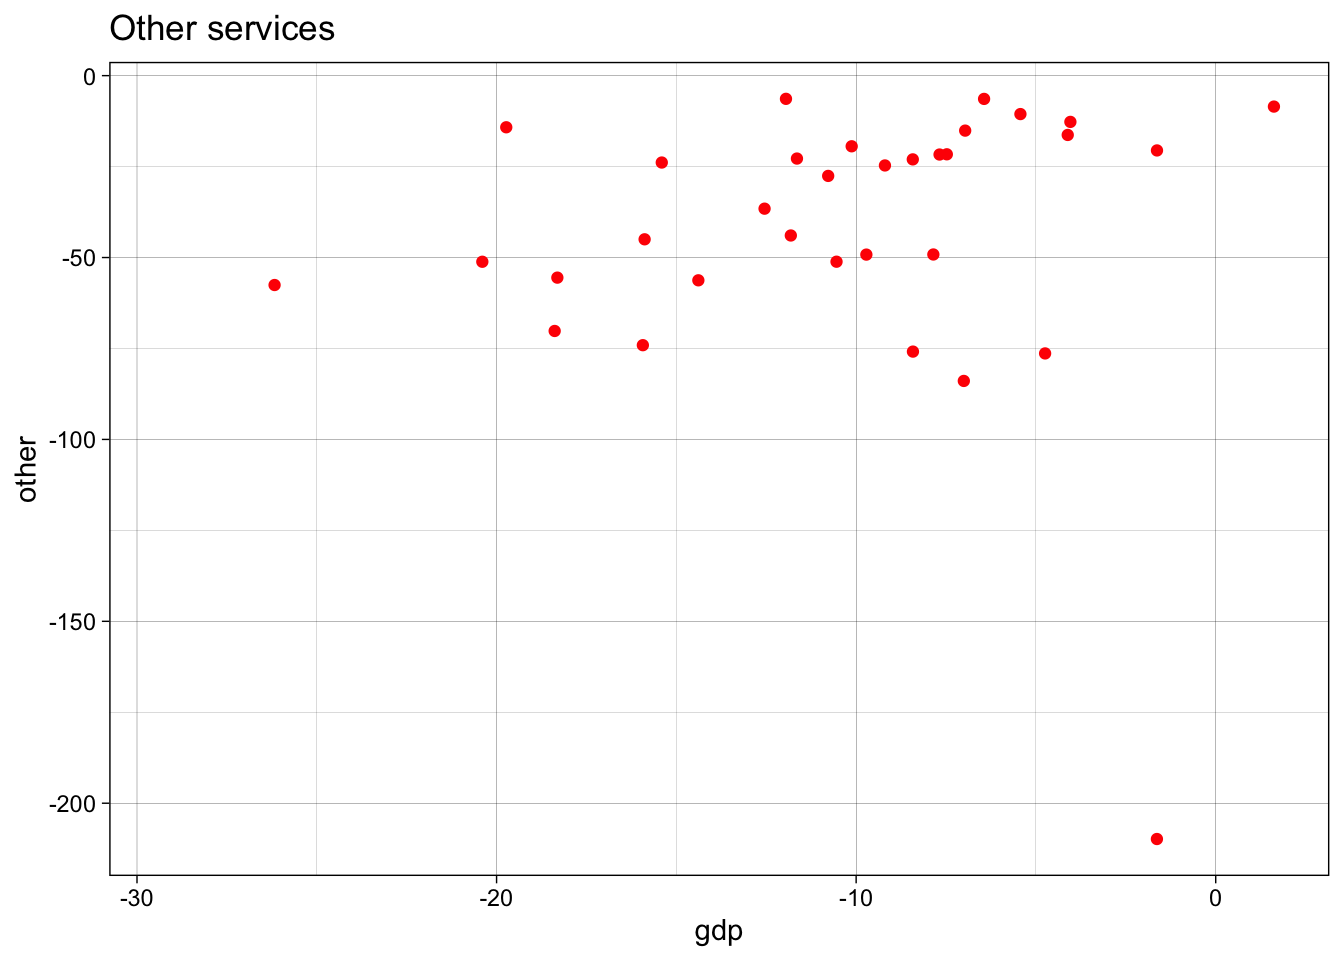
\includegraphics[width=0.33\linewidth]{Morocco_GDP_prediction_files/figure-latex/unnamed-chunk-1-2}
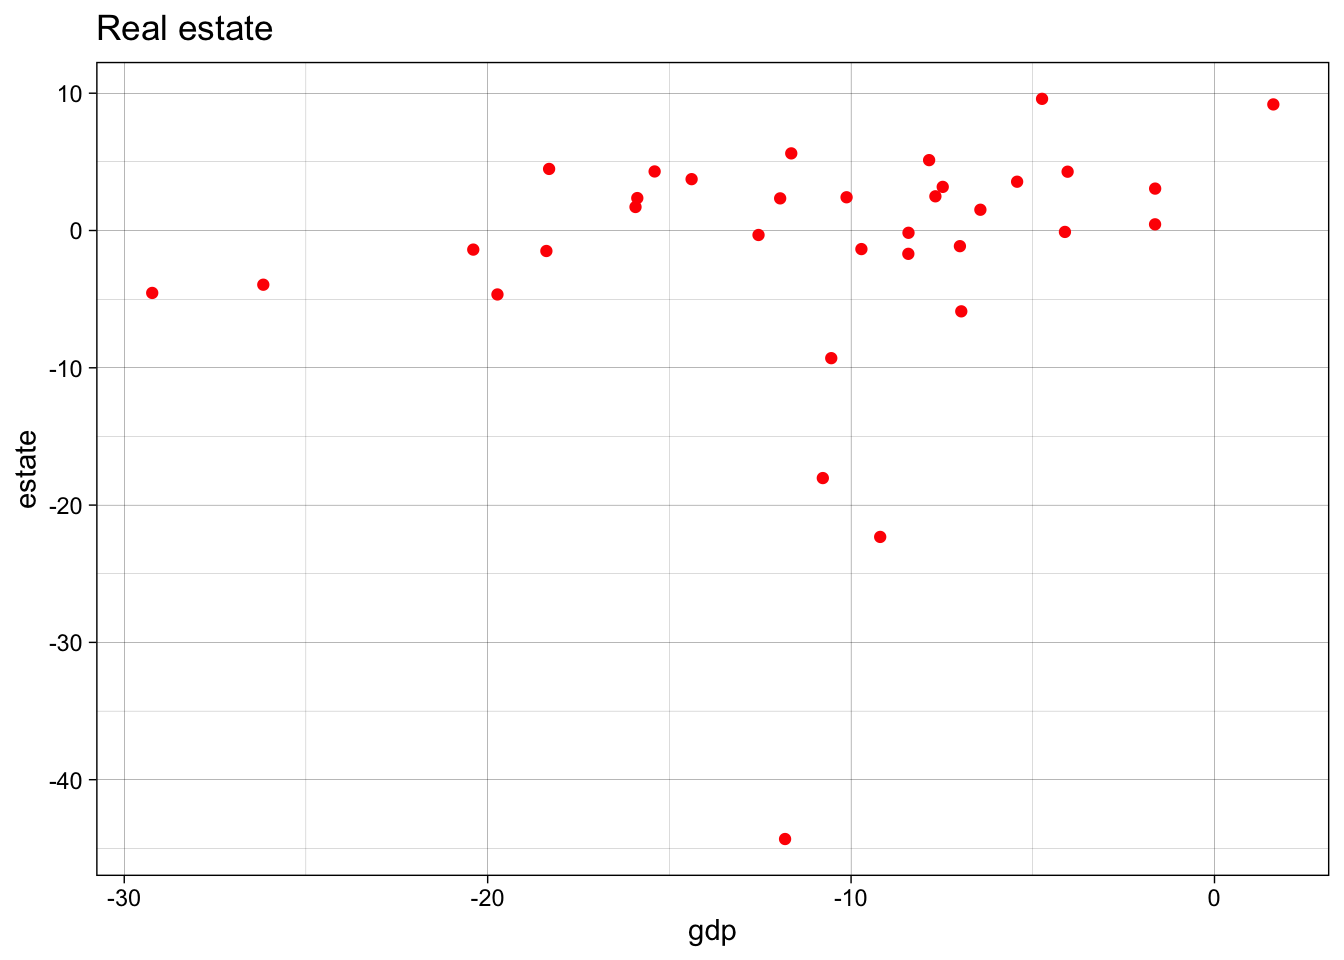
\includegraphics[width=0.33\linewidth]{Morocco_GDP_prediction_files/figure-latex/unnamed-chunk-1-3}

Given the bunching in Agriculture which is the result of a far outlying
value in Ireland, we remove that observation and another one from
Estonia. We also remove the outlier in Other Services (Ireland again)
and a final one in Estate.

Perhaps later we can try a more rigorous method of outlier removal.

We can see that this has led to a more linear shape, meaning better
estimates can be made from the data.

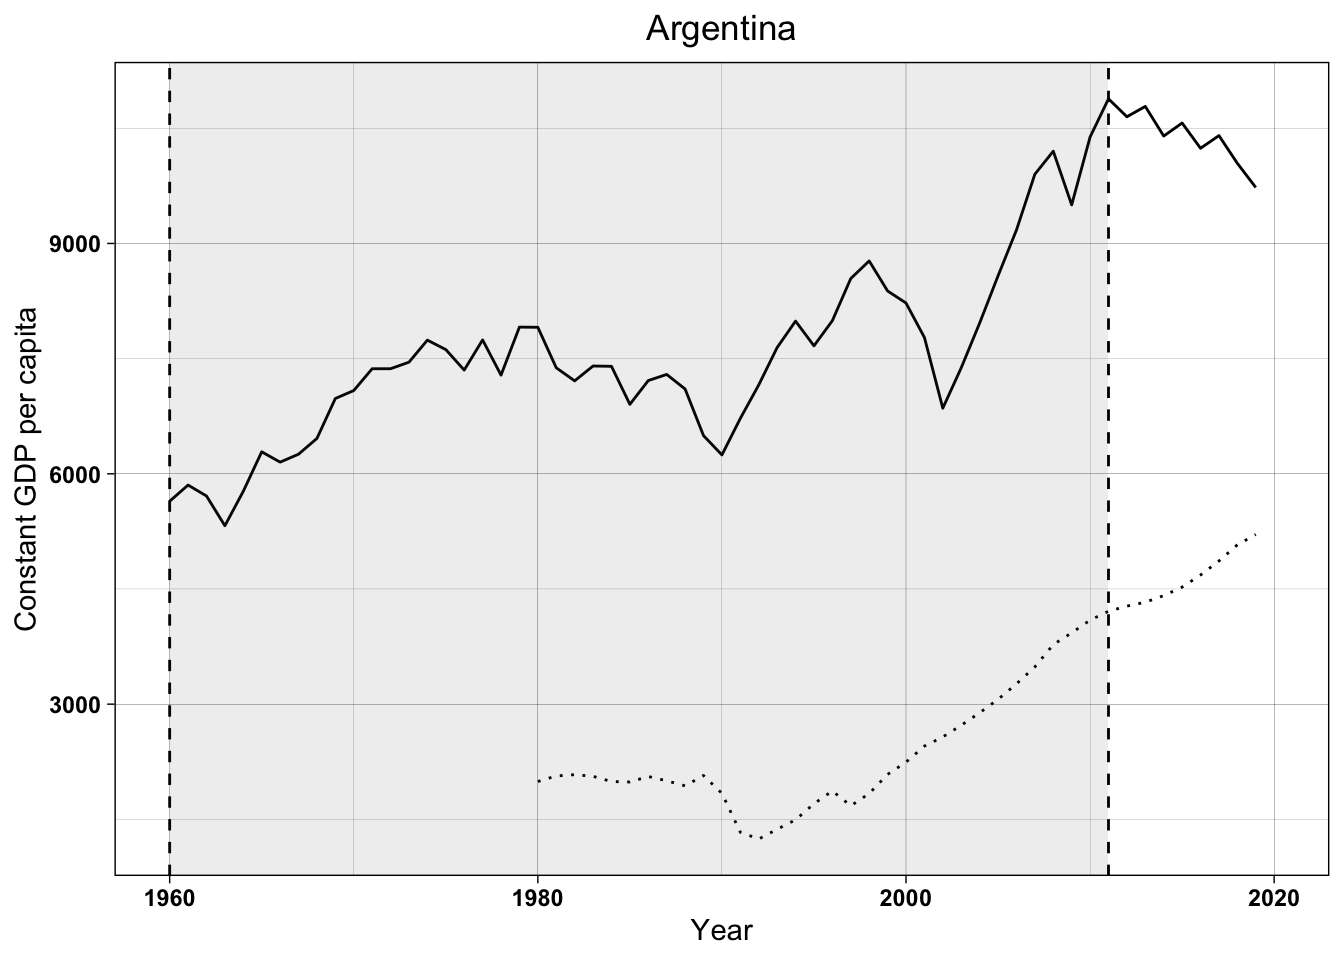
\includegraphics[width=0.33\linewidth]{Morocco_GDP_prediction_files/figure-latex/unnamed-chunk-2-1}
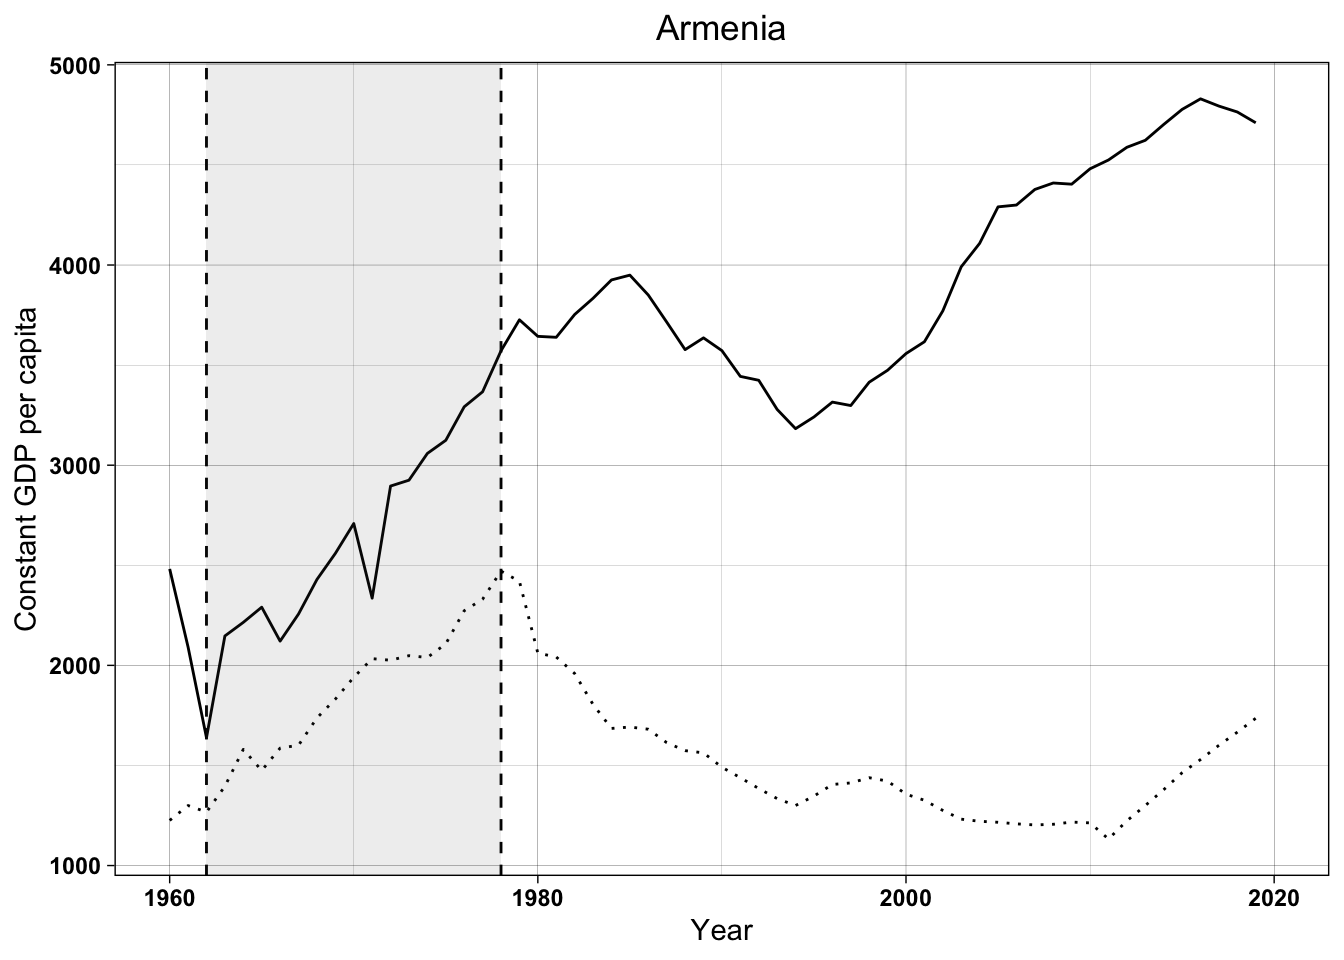
\includegraphics[width=0.33\linewidth]{Morocco_GDP_prediction_files/figure-latex/unnamed-chunk-2-2}
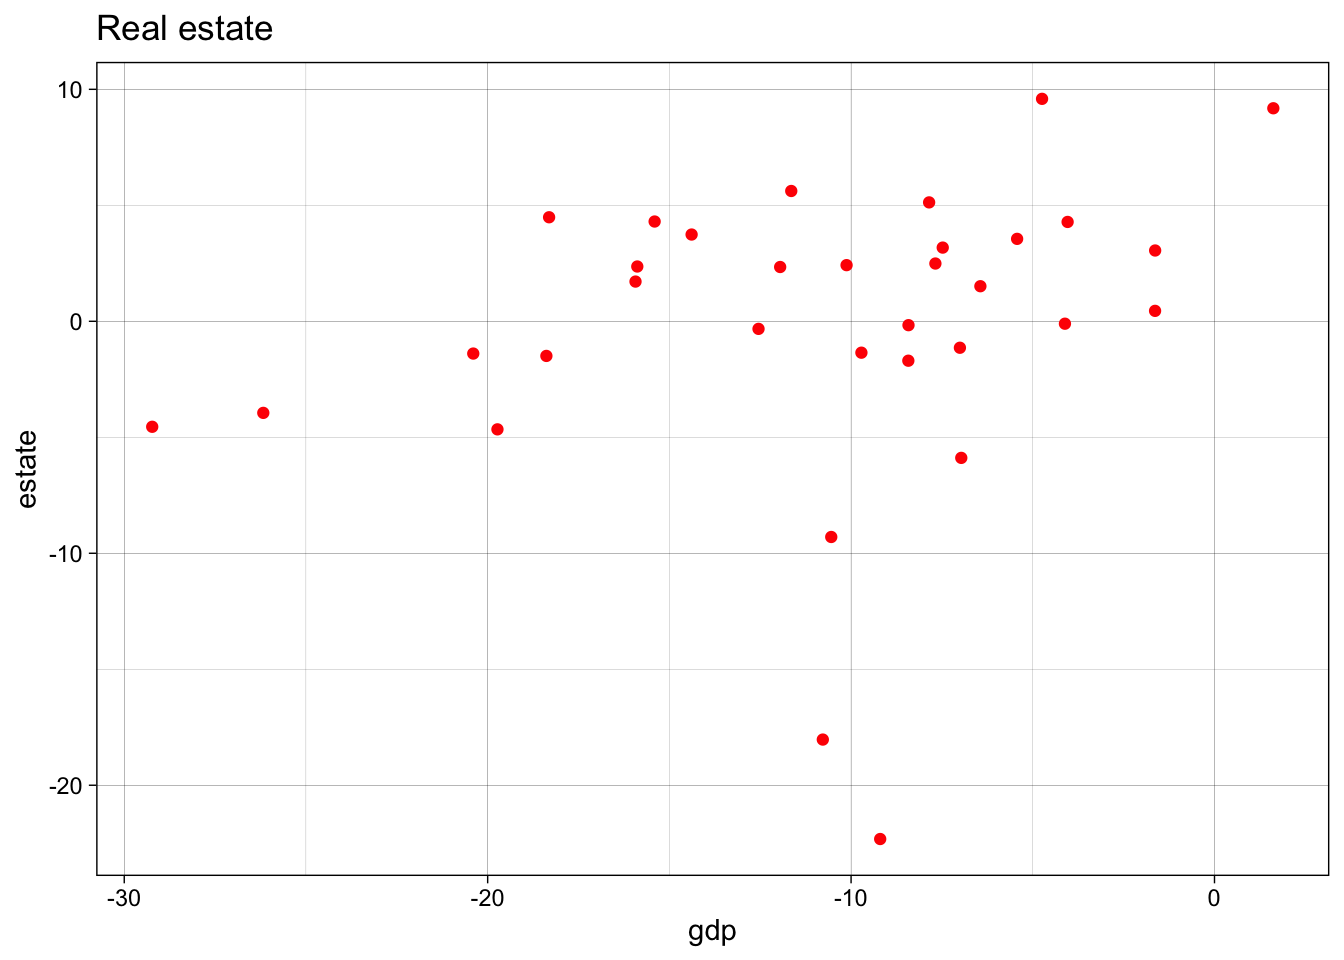
\includegraphics[width=0.33\linewidth]{Morocco_GDP_prediction_files/figure-latex/unnamed-chunk-2-3}

Re-running the model with these values gone:

\begin{Shaded}
\begin{Highlighting}[]
\NormalTok{full.set<-}\KeywordTok{lm}\NormalTok{(gdp }\OperatorTok{~}\StringTok{ }\NormalTok{agri }\OperatorTok{+}\StringTok{ }\NormalTok{cons }\OperatorTok{+}\StringTok{ }\NormalTok{trade }\OperatorTok{+}\StringTok{ }\NormalTok{fin }\OperatorTok{+}\StringTok{ }\NormalTok{industry }\OperatorTok{+}\StringTok{ }\NormalTok{info }\OperatorTok{+}\StringTok{ }\NormalTok{manuf }\OperatorTok{+}\StringTok{ }\NormalTok{other }\OperatorTok{+}\StringTok{ }\NormalTok{tech }\OperatorTok{+}\StringTok{ }\NormalTok{public }\OperatorTok{+}\StringTok{ }\NormalTok{estate }\OperatorTok{+}\StringTok{ }\NormalTok{services, }\DataTypeTok{data=}\NormalTok{tot.wide)}

\KeywordTok{summary}\NormalTok{(full.set)}
\end{Highlighting}
\end{Shaded}

\begin{verbatim}
## 
## Call:
## lm(formula = gdp ~ agri + cons + trade + fin + industry + info + 
##     manuf + other + tech + public + estate + services, data = tot.wide)
## 
## Residuals:
##      Min       1Q   Median       3Q      Max 
## -1.65960 -0.53745 -0.02484  0.45841  1.82651 
## 
## Coefficients:
##               Estimate Std. Error t value Pr(>|t|)   
## (Intercept) -1.0221124  0.7720129  -1.324  0.20304   
## agri         0.0328247  0.0297094   1.105  0.28461   
## cons         0.0007845  0.0187253   0.042  0.96707   
## trade        0.1243877  0.0454437   2.737  0.01404 * 
## fin          0.1113031  0.0394554   2.821  0.01177 * 
## industry     0.1988555  0.0566331   3.511  0.00268 **
## info         0.1439704  0.0449034   3.206  0.00518 **
## manuf        0.0208102  0.0367099   0.567  0.57820   
## other        0.0055643  0.0116844   0.476  0.63999   
## tech         0.0458079  0.0369321   1.240  0.23170   
## public       0.0483939  0.0856708   0.565  0.57953   
## estate       0.0526661  0.0524092   1.005  0.32903   
## services     0.1960155  0.1967376   0.996  0.33306   
## ---
## Signif. codes:  0 '***' 0.001 '**' 0.01 '*' 0.05 '.' 0.1 ' ' 1
## 
## Residual standard error: 1.068 on 17 degrees of freedom
##   (4 observations deleted due to missingness)
## Multiple R-squared:  0.9823, Adjusted R-squared:  0.9698 
## F-statistic: 78.72 on 12 and 17 DF,  p-value: 1.889e-12
\end{verbatim}

\hypertarget{prediction}{%
\subsubsection{Prediction}\label{prediction}}

The model has improved slightly for GDP with a higher R-squared and more
significant variables. Now we can see how well it predicts GDP for
Morocco. We use only the sectors that are found in the data we have for
Morocco, build the model with them and run the training model. Then we
add in Morocco as the validation portion to see how well this model
predicts GDP.

\begin{Shaded}
\begin{Highlighting}[]
\NormalTok{train<-}\KeywordTok{lm}\NormalTok{(gdp }\OperatorTok{~}\StringTok{ }\NormalTok{agri }\OperatorTok{+}\StringTok{ }\NormalTok{trade }\OperatorTok{+}\StringTok{ }\NormalTok{fin }\OperatorTok{+}\StringTok{ }\NormalTok{manuf }\OperatorTok{+}\StringTok{ }\NormalTok{other }\OperatorTok{+}\StringTok{ }\NormalTok{tech }\OperatorTok{+}\StringTok{ }\NormalTok{public }\OperatorTok{+}\StringTok{ }\NormalTok{services, }\DataTypeTok{data=}\NormalTok{tot.wide)}

\KeywordTok{predict}\NormalTok{(train, }\DataTypeTok{newdata =}\NormalTok{ mar.gdp, }\DataTypeTok{interval =} \StringTok{"prediction"}\NormalTok{)}
\end{Highlighting}
\end{Shaded}

\begin{verbatim}
##         fit       lwr       upr
## 1 -11.32872 -19.49619 -3.161243
\end{verbatim}

The fitted value shows that this model predicts Morocco's GDP to be at
\textbf{-11.32872}.

This is not far from the actual observed value of \textbf{-9.3424}. This
could mean that this model does a decent job of representing Covid's
impact by sector and could be applied to other applications in the
future.

Next steps:

\begin{itemize}
\tightlist
\item
  Running this for a number of countries to see how it predicts those
\item
  Improving prediction through adding more samples
\item
  Robustness checks and further evaluation of predictive ability
\end{itemize}

\end{document}
